% coding:utf-8

\section{Aufgaben}
Auf den folgenden Seiten finden Sie viele verschiedene Aufgaben die
Sie während dem Kurs in Angriff nehmen können. Beachten Sie hierzu 
bitte die folgenden Hinweise:

\begin{enumerate}
\item Sie müssen nicht alle Aufgaben im Kurs lösen.
\item Sie können die Kursunterlagen nach Hause nehmen und dort weiter Programmieren. 
\item Die Aufgaben sind so gestellt, dass Sie eine nach der anderen lösen 
müssen. 
\item Sie müssen die Aufgaben nicht alleine lösen sondern können in Teams bearbeiten.
\end{enumerate}

\noindent
Hier sehen Sie eine Übersicht der Aufgaben:

% Hier Tabelle mit Aufgaben einfügen
\begin{table}[h!]
\centering
\begin{tabular}{cll}
\textbf{Aufgabe} & \textbf{Themen} & \textbf{Schwierigkeit} \\ 
\hline
1 & Pausen, Ausgaben, absolute Sprünge & einfach \\ 
2 & Pausen, Ausgaben, absolute Sprünge & einfach \\ 
3 & Pausen, Ausgaben, absolute Sprünge & einfach \\ 
4 & Pausen, Ausgaben, relative Sprünge & einfach \\ 
5 & Eingaben, einfache Verzweigungen & mittel \\ 
6 & Eingaben, geschachtelte Verzweigungen & mittel \\ 
7 & Zählerschlaufen, Zeitberechnung & mittel  \\ 
8 & Zählerschlaufen, Theorie zu Variablen & mittel \\ 
9 & Zählerschlaufen, Variablen & schwer \\ 
\end{tabular} 
\caption{Übersicht der Aufgaben}
\end{table}

\noindent
Wer gerne weitere Aufgabe haben möchte, kann sich beim Instruktor melden.

\newpage
\subsection{Aufgabe 1}
Betrachten Sie nochmals das Testprogramm.
\lstinputlisting[label=Testprogramm, caption=Testprogramm]{../listings/test.bas}

\noindent

\begin{enumerate}[label=(\alph*)]
	\item Versuchen Sie zu zweit oder zu dritt zu verstehen, wie das
	Programm arbeitet.
	\item Versuchen Sie alleine das Programm langsamer zu machen.
	\item Ändern Sie das Programm so, dass eine andere LED blinkt.
\end{enumerate}

\ifteacher
\newpage
\subsection{Lösung zu Aufgabe 1}
\begin{enumerate}[label=(\alph*)]
	\item Die einzelnen Zeilen im Programm sind jeweils Dokumentiert
	mit einem Kommentar. Kommentare erkennt man daran, dass diese mit
	einem \lstinline{'} eingeleitet und in der Entwicklungsumgebung
	grün dargestellt werden. Alles was rechts von diesem 
	Zeichen steht, ist ein Kommentar und wird vom Computer ignoriert.\\
	\textbf{Beispiel:} In der Zeile 3 steht der Kommentar 
	\lstinline{'LED 0 einschalten}.
	\begin{itemize}
		\item Als erstes wird mittels \lstinline{HIGH 0} die LED 0 
		eingeschaltet.
		\item Danach wird eine Pause von 500 Millisekunden 
		(\nicefrac{1}{2} Sekunde) mit \lstinline{PAUSE 500} eingelegt.
		\item Mit \lstinline{LOW 0} wird die LED 0 wieder ausgeschaltet.
		\item Erneut wird wieder mit \lstinline{PAUSE 500} eine halbe
		Sekunde lang nichts gemacht.
		\item Mit \lstinline{GOTO start} wird als nächstes die Zeile
		im Programm ausgeführt wo das Label \lstinline{start} steht
		(d.h. in Zeile 3). Durch das \lstinline{GOTO start} wird das
		Programm unendlich oft wiederholt, da es am Ende immer an den
		Anfang (\lstinline{start}) springt.
	\end{itemize}
	\item Um das Programm langsamer zu machen, muss die Pausenzeit
	verlängert werden. Man könnte diese z.B. auf 1000ms setzen.
	\lstinputlisting[label=, caption=]{../listings/test-slow.bas}
	\item Um eine andere LED blinken zu lassen muss die Nummer hinter 
	\lstinline{HIGH} und \lstinline{LOW} geändert werden, z.B. auf 7.
	\lstinputlisting[label=,caption=]{../listings/test-other.bas}
\end{enumerate}
\fi

\newpage
\subsection{Aufgabe 2}
Betrachten Sie folgendes Programm.

\lstinputlisting[label=, caption= ]{../listings/halfknight.bas}

\begin{enumerate}[label=(\alph*)]
	\item Versuchen Sie zu erraten was das Programm macht.
	\item Laden Sie das Programm auf Ihr \verb!BASIC Stamp! und überprüfen Sie 
	Ihre Vermutung.
	\item Versuchen Sie ein Programm zu schreiben,
	welches genau umgekehrt läuft.
\end{enumerate}

\ifteacher
\newpage
\subsection{Lösung zu Aufgabe 2}
\begin{enumerate}[label=(\alph*)]
	\item Das Programm schaltet eine LED nach der anderen ein und wieder
	aus. Es beginnt dabei bei der LED 0 und nach der LED 7 macht es von
	vorne weiter.
	\item ~
	\item Um eine LED nach der anderen ein- und ausschalten zu lassen 
	von der LED 7 beginnend zur LED 0 müsste wie folgt aussehen.
	\lstinputlisting[label=,caption=]{../listings/halfknight-reverse.bas}
\end{enumerate}
\fi

\newpage
\subsection{Aufgabe 3}
Können Sie sich erinnern an die alte Fernsehserie \emph{Knight Rider}?
In dieser gab es ein Auto Namens Kit welches einen Computer eingebaut hatte.
Dieses war sehr berühmt für sein cooles Frontlicht welches immer hin und her
lief.

\begin{enumerate}[label=(\alph*)]
	\item Versuchen Sie ein Programm zu schreiben, welches die LEDs
	wie bei Kit hin und her blinken lässt. Als Hilfe haben Sie unten 
	eine Zeichnung die den Ablauf nochmals beschreibt. \\
	\footnotesize
	Tipp: Sie haben in der Aufgabe 2 bereits etwas ähnliches programmiert.
	\normalsize
	\item Vergleichen Sie Ihre Lösung mit der von anderen und besprechen
	Sie diese zusammen.
\end{enumerate}

\vfill
\begin{figure}[h!]
	\centering
	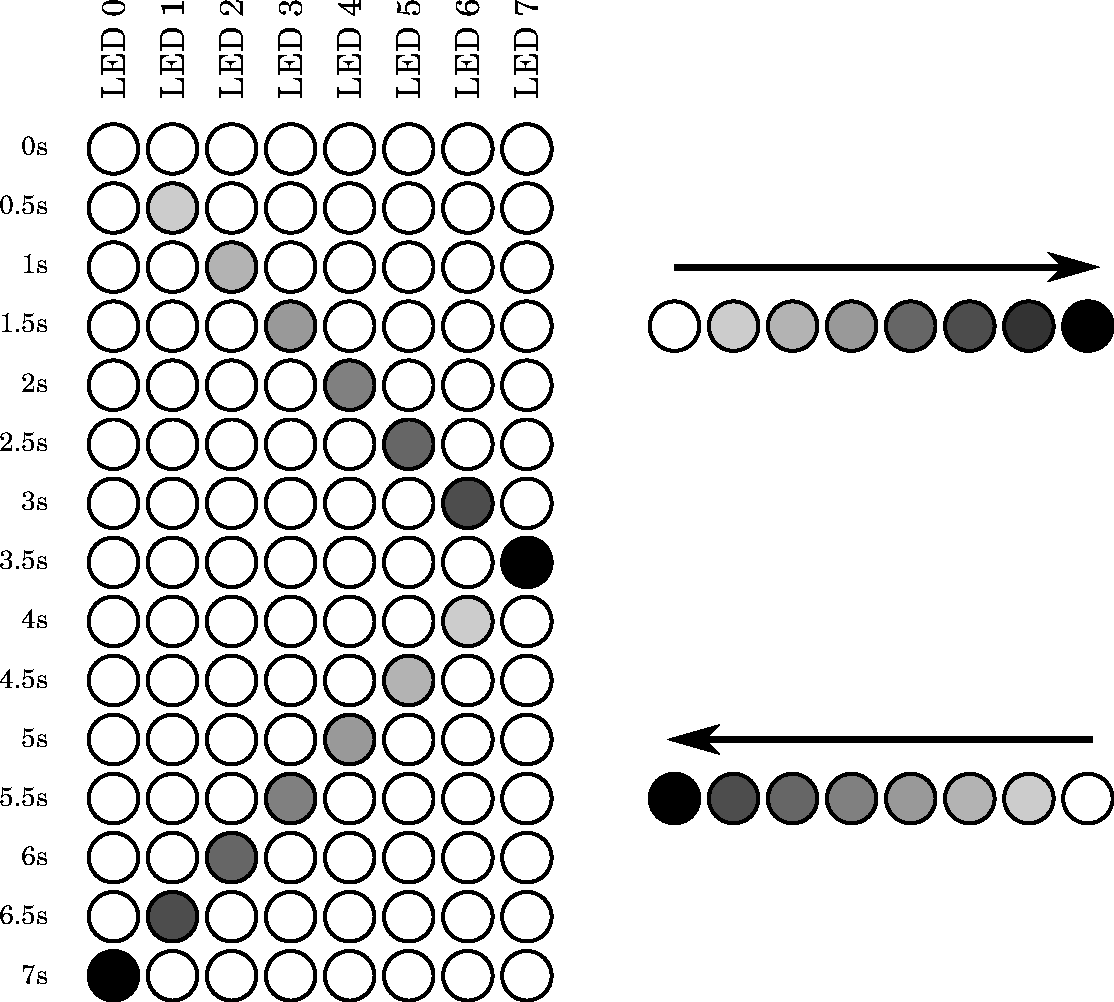
\includegraphics[scale=0.6]{../pictures/knightrider.pdf}
	\caption{Hilfszeichnung zum Knight Rider}
\end{figure}
\vfill

\ifteacher
\newpage
\subsection{Lösung zu Aufgabe 3}
\begin{enumerate}[label=(\alph*)]
	\item Wir können das Programm aus der vorhergehenden Aufgabe nehmen
	und diese einfach erweitern.
	\lstinputlisting[label=,caption=]{../listings/knightrider-simple.bas}
\end{enumerate}
\fi

\newpage
\subsection{Aufgabe 4}
In der Aufgabe 3 haben Sie vielleicht bemerkt, dass sich vieles im 
Programm wiederholt. Teile die sich in Programmen wiederholen sind
wo immer möglich zu vermeiden, denn sie machen den Code schwerfällig.
Was das heisst merken Sie bestimmt in der folgenden Aufgabe.

\begin{enumerate}[label=(\alph*)]
	\item Verändern Sie Ihr Programm aus Aufgabe 3 so, dass es doppelt
	so schnell wird.
	\item Was ist Ihnen aufgefallen beim lösen der Aufgabe (a)?
	\item Nehmen Sie Ihr Programm aus Aufgabe (4a) und machen Sie folgende
	Anpassung:\\
	\begin{itemize}
		\item Ersetzten Sie jede Zeile in der 
		\begin{lstlisting}
		PAUSE
		\end{lstlisting}
		vorkommt mit der Zeile
		\begin{lstlisting}
		GOSUB warten
		\end{lstlisting}
		\item Fügen Sie ganz am Ende des Programms die folgenden 
		zwei Zeilen hinzu:
		\begin{lstlisting}
warten:  PAUSE 500
         RETURN
		\end{lstlisting}
	\end{itemize}
	\item Versuchen Sie zu erraten was das Programm nun machen wird.
	\item Laden Sie das Programm auf Ihr \verb!BASIC Stamp! und beobachten
	Sie was passiert.
	\item Ändern Sie die Geschwindigkeit des Lauflichts so, dass es 
	Ihnen gefällt.
\end{enumerate}

\ifteacher
\newpage
\subsection{Lösung zu Aufgabe 4}
\begin{enumerate}[label=(\alph*)]
	\item Um das Programm schneller zu machen muss lediglich die Pausenzeit
	kleiner gewählt werden. Zum Beispiel auf 100ms mit
	\lstinline{PAUSE 100}.
	\item Ihnen sollte aufgefallen sein, dass die Veränderung der Pausenzeit
	eine einfache Aufgabe ist, jedoch sehr mühsam da man diese an vielen 
	Stellen im Programm von Hand ändern muss.


\end{enumerate}
\fi

\newpage
\subsection{Aufgabe 5}
Betrachten Sie folgendes Programm.

\lstinputlisting[label=, caption=]{../listings/button.bas}

\begin{enumerate}[label=(\alph*)]
	\item Versuchen Sie zu erraten, was das
	Programm macht.
	\item Laden Sie das Programm auf Ihr \verb!BASIC Stamp! und
	experimentieren Sie. Was stellen Sie fest?
\end{enumerate}

\ifteacher
\newpage
\subsection{Lösung zu Aufgabe 5}
\begin{enumerate}[label=(\alph*)]
	\item Die Taste 0 wird als Eingabe definiert. Ist diese gedrückt
	beim Label \lstinline{start} so springt das Programm zum Label 
	\lstinline{abc}. Dort angelangt wird die LED 4 eingeschaltet mit
	\lstinline{HIGH 4}. Solange die Taste gedrückt ist, bleibt die
	LED 4 eingeschaltet, denn es springt zu \lstinline{start} und
	gleich danach zu \lstinline{abc}. Lässt man die Taste nun los
	geht es nicht zu \lstinline{abc} sondern einfach zur nächsten Zeile
	im Programm. Dort steht dann \lstinline{LOW 4} was die LED 4
	ausschaltet.

	\textbf{Zusammengefasst:}\\
	Drückt man die Taste 0, so leuchtet die LED 4.
	Lässt man sie los, so leuchtet sie nicht.
	\item Drückt man eine Taste, so leuchtet immer die zugehörige LED.
	Das hat nichts mit dem Programm zu tun sondern ist etwas spezielles
	am Board selbst.
\end{enumerate}
\fi

\newpage
\subsection{Aufgabe 6}
In der Aufgabe 5 haben Sie gelernt wie man eine Eingabe macht und darauf
reagieren kann mit einer Ausgabe.

\begin{enumerate}[label=(\alph*)]
	\item Nehmen Sie das Programm aus Aufgabe 5 als Grundlage und
	erstellen Sie ein neues Programm, welches für jeden Taster jeweils
	eine LED leuchten lässt wie es in der Leuchttabelle beschrieben ist.
	Die LEDs sollen nur so lange leuchten wie die Tasten gedrückt sind.

	\begin{table}[h!]
		\centering
		\begin{tabular}{lcl}
			\textbf{Eingabe} & & \textbf{Ausgabe} \\ \hline
			Taste 0 = 1 
				& $ \quad \rightarrow \quad$ 
					& LED 4 leuchtet \\
			Taste 1 = 1 
				& $ \quad \rightarrow \quad $ 
					& LED 5 leuchtet \\
			Taste 2 = 1 
				& $ \quad \rightarrow \quad $ 
					& LED 6 leuchtet \\
			Taste 3 = 1 & $\rightarrow$ & LED 7 leuchtet \\
		\end{tabular}
		\caption{Leuchttabelle zu (6a)}	
	\end{table}
	
	\item Ändern Sie das Programm aus Aufgabe (a) so, dass jeweils zwei
	Tasten gedrückt werden müssen um eine LED leuchten zu lassen.

	\begin{table}[h!]
		\centering
		\begin{tabular}{lcl}
			\textbf{Eingabe} & & \textbf{Ausgabe} \\ \hline
			Taste 0 = 1 und Taste 1 = 1 
				& $ \quad \rightarrow \quad $ 
					& LED 5 leuchtet \\
			Taste 2 = 1 und Taste 3 = 1
				& $ \quad \rightarrow \quad $ 
					& LED 7 leuchtet \\
		\end{tabular}
		\caption{Leuchttabelle zu (6b)}	
	\end{table}
	\item \* Wie viele Kombinationen von Eingaben gibt es mit vier 
	Tastern?
\end{enumerate}

\ifteacher
\newpage
\subsection{Lösung zu Aufgabe 6}
\begin{enumerate}[label=(\alph*)]
	\item Einerseits müssen wir mehr Taster definieren und andererseits
	müssen wir mehr Sprungsstellen definieren.
	\lstinputlisting[label=,caption=]{../listings/button-quad.bas}
	\item Es muss zwei mal nach einander angefragt werden ob die Tasten
	gedrückt sind. Zudem können die Tasten in verschiedenen Reihenfolgen
	gedrückt werden.
	\lstinputlisting[label=,caption=]{../listings/button-double.bas}
	\item Es gibt insgesamt 16 Kombinationen, denn man hat vier Taster
	mit jeweils zwei Zuständen (Ein/Aus) und somit 
	$2^4=2 \cdot 2 \cdot 2 \cdot 2=16$
	Kombinationen.
\end{enumerate}
\fi

\newpage
\subsection{Aufgabe 7}\label{timing-problem}
Betrachten Sie folgendes Programm.
\lstinputlisting[label=,caption=]{../listings/counter.bas}

\begin{enumerate}[label=(\alph*)]
\item Versuchen Sie zu erraten was das Programm macht.
\item Tippen Sie das Programm ab und laden es auf Ihr \lstinline{BASIC Stamp}.
\item Erweitern Sie das Programm so, dass die LED 7 für 15 Sekunden blinkt, wenn die 
Taste 0 gedrückt wird. Das Blinken soll dabei einen Takt von 300 Millisekunden haben.
\end{enumerate}

\ifteacher
\newpage
\subsection{Lösung zu Aufgabe 7}
\begin{enumerate}[label=(\alph*)]
\item \dots
\item \dots 
\item Ein Zyklus soll 15 Sekunden dauern. In solch einen Zyklus soll eine gerade
Anzahl Pausen mit 300 Millisekunden stattfinden. Cooles Problem denn wir können 
einfach Algebra verwenden:
\[  \text{15 Sekunden} = x \cdot 2 \cdot \text{Pausenzeit} \]
\[  15 = x \cdot 2 \cdot 0.3 \qquad |\div 2 \]
\[  \frac{15}{2} = x \cdot 0.3 \qquad |\div 0.3 \]
\[ \frac{15}{2 \cdot 0.3} = x  \qquad |\Leftrightarrow x \]
\[ x = \frac{15}{2 \cdot 0.3} \]
\[ x = \frac{15}{0.6} \]
\[ x = 25 \]
Nun wissen wir, dass wir 25 Zyklen brauchen. Da wir bei 0 und nicht bei 1 zu Zählen 
beginnen, müssen wir 1 abziehen d.h. wie schreiben \lstinline{FOR B2 = 0 TO 25}.
\lstinputlisting[label=,caption=]{../listings/counter-blink.bas}
\end{enumerate}
\fi

\newpage
\subsection{Aufgabe 8}
Betrachten Sie folgendes Programm.
\lstinputlisting[label=,caption=]{../listings/variable-simple.bas}

\begin{enumerate}[label=(\alph*)]
\item Lesen Sie die Theorie zum Thema Platzhalter im Kapitel \ref{Platzhalter}.
\item Versuchen Sie mit Hilfe der Theorie aus (a) das Programm zu verstehen.
\item Laden Sie das Programm auf Ihr \verb|BASIC Stamp| und untersuchen Sie, 
ob Ihre Annahmen stimmen.
\end{enumerate}

\ifteacher
\newpage
\subsection{Lösung zu Aufgabe 8}
\begin{enumerate}[label=(\alph*)]
\item \dots
\item \dots
\item \dots
\end{enumerate}
\fi

\newpage
\subsection{Aufgabe 9}
Betrachten Sie folgendes Programm.
\lstinputlisting{../listings/auto-halfknight.bas}

\begin{enumerate}[label=(\alph*)]
\item Versuchen Sie zu verstehen was das Programm macht.
\item Laden Sie das Programm auf Ihr \verb|BASIC Stamp| und untersuchen Sie,
ob Ihre Annahmen stimmen.
\item Entwickeln Sie ein Knight Rider Lauflicht mit Variablen und 
\lstinline{FOR ... NEXT} Schlaufen wie im Beispielcode.
\item Erweitern Sie das Programm aus (c) so, 
dass zwei Knight Rider entgegengesetzt laufen.\\
\footnotesize
Tipp: Wenn zwei Knight Rider entgegenlaufen, so sind immer
die folgenden LEDs gleichzeitig ein:
\begin{table}[h!]
\centering
\begin{tabular}{ccc}
\vdots & \vdots \\
LED 0 & LED 7 \\
LED 1 & LED 6 \\
LED 2 & LED 5 \\
LED 3 & LED 4 \\
LED 4 & LED 3 \\
LED 5 & LED 2 \\
LED 6 & LED 1 \\
LED 7 & LED 0 \\
\vdots & \vdots  \\
\end{tabular}
\caption{Hilfstabelle zum entgegenlaufenden Knight Rider}
\end{table}
\normalsize
\end{enumerate}

\ifteacher
\newpage
\subsection{Lösung zu Aufgabe 9}
\begin{enumerate}[label=(\alph*)]
\item \dots
\item \dots
\item Code \\ \lstinputlisting[label=,caption=]{../listings/better-knight.bas}
\item Code \\ \lstinputlisting[label=,caption=]{../listings/double-knight.bas}
\end{enumerate}
\fi
